%%%%%%%%%%%%%%%%%%%%%%%%%%INICIO EJERCICIO 8a %%%%%%%%%%%%%%%%%%%%%%%%%%%
\textbf{Solución a.}\\
% La tabla irá centrada
\begin{center}
	\renewcommand{\arraystretch}{1.5}% Márgenes de las celdas
	% Creación de la cuadrícula de 2 columnas
	\begin{longtable}[H]{|c|c|}
		% Creamos una línea horizontal
		\hline
		% Definimos el color de la primera fila
		\rowcolor[HTML]{FFB183} \hline
		%%%%% INICIO ASIGNACIÓN PERÍODO FOCAL %%%%%%%
		%%%%%%%%%% INICIO TÍTULO
		% Lo que se hace aquí es mezclar las 2 columnas en una sola
		\multicolumn{2}{|c|}{\cellcolor[HTML]{FFB183}\textbf{1. Asignación período focal}} \\ \hline
		%%%%%%%%%% FIN TÍTULO
		%%%%% INICIO DECLARACIÓN DE VARIABLES %%%%%%%
		\multicolumn{2}{|c|}{$pf : 0 \; \textit{psv}$} \\ \hline
		%%%%%%%%%% INICIO TÍTULO
		% Lo que se hace aquí es mezclar las 2 columnas en una sola
		\multicolumn{2}{|c|}{\cellcolor[HTML]{FFB183}\textbf{2. Declaración de variables}} \\ \hline

		%%%%%%%%%% FIN TÍTULO
		%%%%%%%%%% INICIO DE MATEMÁTICAS
		\cellcolor[HTML]{FFB183}\textbf{Valores monetarios} & 
		\cellcolor[HTML]{FFB183}\textbf{Valores no monetarios} \\ \hline
		$L = 60{.}000 \; \text{COP}$ & $j = 32\% \; \text{nasv}$ \\ 
		$H = 25{.}000 \; \text{COP}$ & $m = 2 \; \text{psv}$ \\ 
		$ $ & $n = 3 \; \text{pav}$ \\ \hline
		%%%%%%%%%% FIN DE MATEMÁTICAS
		%%%%% FIN DECLARACIÓN DE VARIABLES

		\rowcolor[HTML]{FFB183}
		\hline
		\multicolumn{2}{|c|}{\cellcolor[HTML]{FFB183}\textbf{3. Diagrama de flujo de caja}} \\ \hline
		\multicolumn{2}{|c|}{ 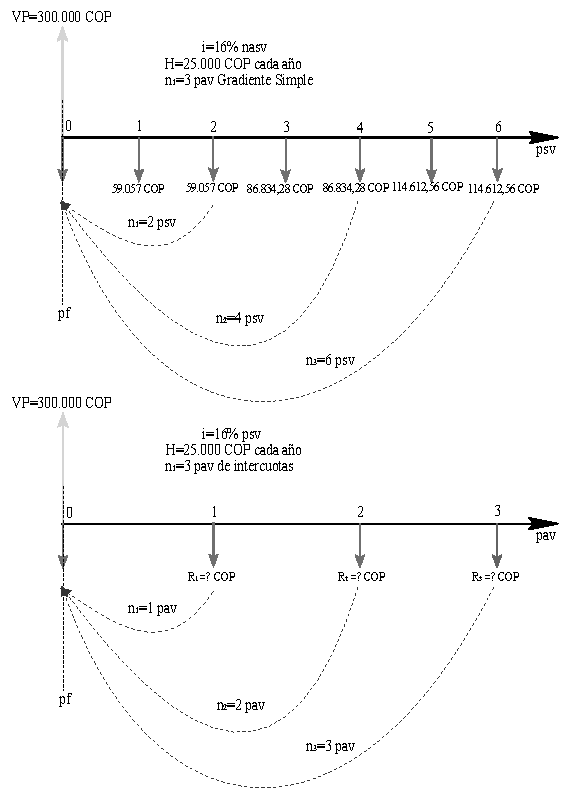
\includegraphics[trim=-78 -5 -78 -5]{7_Capitulo/img/ejemplos/8/8_1.pdf} } \\ \hline
		%%%%% INICIO FLUJO DE CAJA
		\rowcolor[HTML]{FFB183}
		\hline
		\multicolumn{2}{|c|}{\cellcolor[HTML]{FFB183}\textbf{4. Declaración de fórmulas}} \\ \hline
		%%%%%%%%%%%%% FIN INSERCIÓN DE IMAGEN
		%%%%% FIN FLUJO DE CAJA

		\multicolumn{2}{|c|}{ $(1 + i_{1})^{m_1} = (1 + i_{2})^{m_2}$ Equivalente de tasas periódicas vencidas } \\ 
		\multicolumn{2}{|c|}{ $VP = R \frac{1-(1+i)^{-n}}{i}$ Valor presente gradiente aritmético } \\ 
		\multicolumn{2}{|c|}{ $VP = \frac{(1+i)^{-n}-1}{i}$ Valor futuro de serie uniforme vencida } \\ 
		\multicolumn{2}{|c|}{ $R_{n} = R_{1} + (n -1)L$ Valor de un gradiente aritmético en un período \(n\)} \\ \hline

		%%%%%% INICIO DESARROLLO MATEMÁTICO
		\rowcolor[HTML]{FFB183}
		\hline
		%%%%%%%%%% INICIO TÍTULO
		\multicolumn{2}{|c|}{\cellcolor[HTML]{FFB183}\textbf{5. Desarrollo matemático}} \\ \hline
		%%%%%%%%%% FIN TÍTULO
		%%%%%%%%%% INICIO MATEMÁTICAS
		\multicolumn{2}{|c|}{ $(1 + 0{,}16)^{2} = (1 + i)^{1}$ } \\ 
		\multicolumn{2}{|c|}{ $i = 34{,}56\% \; \textit{pav}$ } \\ \hline

		%%%%%%%%%% FIN MATEMÁTICAS
		%%%%%% FIN DESARROLLO MATEMÁTICO
		%%%%%% INICIO RESPUESTA
		\rowcolor[HTML]{FFB183}
		\hline
		%%%%%%%%%% INICIO TÍTULO
		\multicolumn{2}{|c|}{\cellcolor[HTML]{FFB183}\textbf{6. Respuesta}} \\ \hline
		%%%%%%%%%% FIN TÍTULO
		%%%%%%%%%% INICIO RESPUESTA MATEMÁTICA
		\multicolumn{2}{|c|}{ 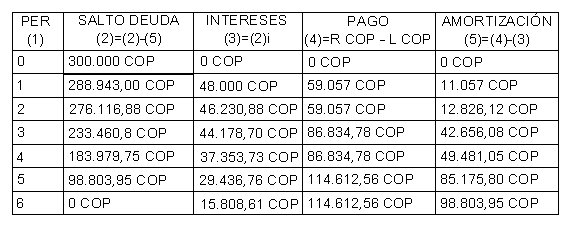
\includegraphics[trim=-78 -5 -78 -5]{7_Capitulo/img/ejemplos/8/8_1_1.pdf} } \\ \hline
	\end{longtable}
	% Se crean dos líneas en blanco para que no quede el siguiente texto tan pegado
	%\newline \newline % USARLO SI CREES QUE ES NECESARIO
\end{center}
%%%%%%%%%%%%%%%%%%%%%%%%%%FIN EJERCICIO 8a %%%%%%%%%%%%%%%%%%%%%%%%%%%
